\section{Validando Experimentos}

\begin{frame}{Problema}
  \begin{itemize}
    \item Qual a diferença entre aprender e decorar?
    \item O experimento está convergindo?
    \item Como saber se o algoritmo realmente generalizou um problema?
  \end{itemize}
\end{frame}

\begin{frame}{Problema}
  \[ \sum_{x_t \in X} (x_t - x_{t}^d) = \varepsilon \]
\end{frame}

\begin{frame}{Validação}
  \begin{block}{Como saber se o algoritmo realmente generalizou um problema?}
  Quando ele consegue se sair bem em dados ainda não vistos.
  \end{block}

  \pause

  \begin{itemize}
    \item Separe uma parte dos dados para teste.
    \item Separe uma parte dos dados de treino para validar o próprio treinamento.
  \end{itemize}

  \begin{figure}[t]
    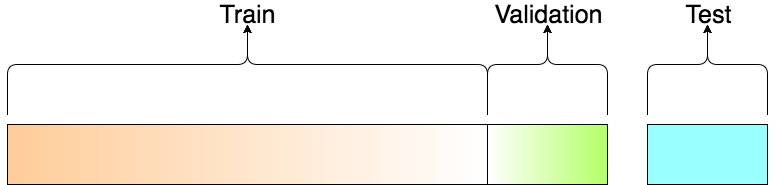
\includegraphics[width=\textwidth]{validation.png}
    \centering
  \end{figure}

\end{frame}

\begin{frame}{Validação Cruzada (K-Fold CV)}
  \begin{block}{Problemas com o método anterior}
    \begin{itemize}
      \item A escolha dos dados pra validação depende muita de sorte.
    \end{itemize}
  \end{block}

  \pause

  \begin{figure}[t]
    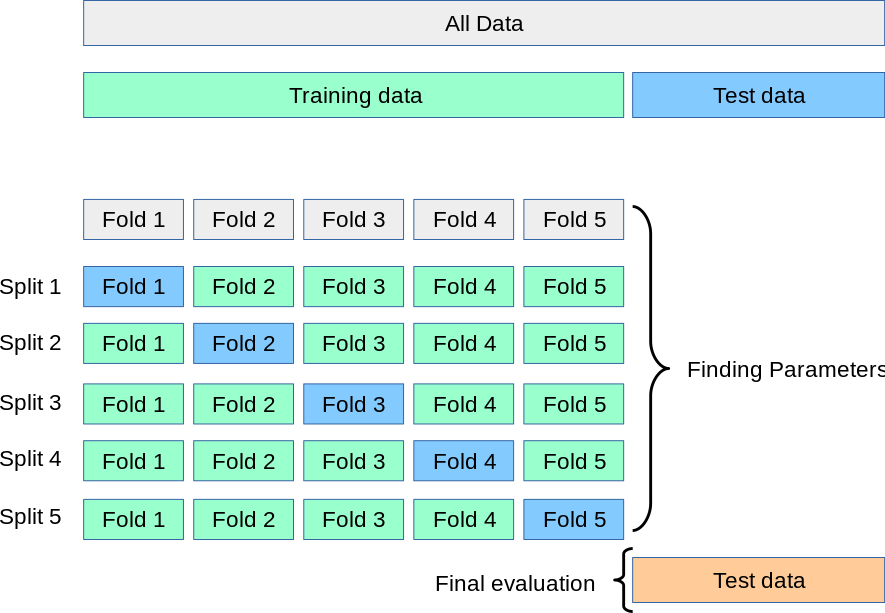
\includegraphics[width=0.6\textwidth]{cross_validation.png}
    \caption{5-Fold cross validation, Fonte: \href{https://scikit-learn.org/stable/modules/cross_validation.html}{scikit-learn}.}
    \centering
  \end{figure}

\end{frame}

\begin{frame}{Monte Carlo cross-validation}
  \begin{figure}[t]
    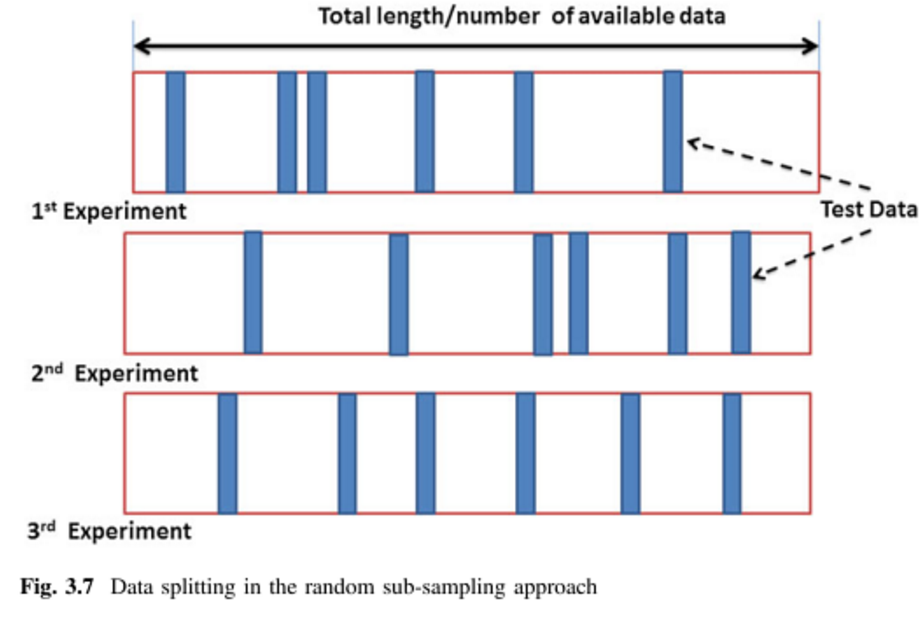
\includegraphics[width=0.8\textwidth]{monte_carlo.png}
    \centering
  \end{figure}
\end{frame}

\begin{frame}{Overfitting}

  \begin{figure}[t]
    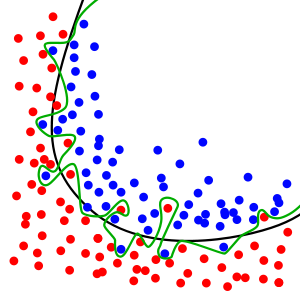
\includegraphics[width=0.6\textwidth]{overfitting.png}
    \caption{Fonte: \href{https://en.wikipedia.org/wiki/Overfitting}{Wikipedia}.}
    \centering
  \end{figure}

\end{frame}

\begin{frame}{Regularização}

\begin{block}{}
  \[ \min \left(\sum_{x_t \in X} (x^\ast_t - x^d_t) + \norm{P} \right) \]
\end{block}

\end{frame}
